\documentclass[11pt,]{article}
\usepackage{lmodern}
\usepackage{amssymb,amsmath}
\usepackage{ifxetex,ifluatex}
\usepackage{fixltx2e} % provides \textsubscript
\ifnum 0\ifxetex 1\fi\ifluatex 1\fi=0 % if pdftex
  \usepackage[T1]{fontenc}
  \usepackage[utf8]{inputenc}
\else % if luatex or xelatex
  \ifxetex
    \usepackage{mathspec}
  \else
    \usepackage{fontspec}
  \fi
  \defaultfontfeatures{Ligatures=TeX,Scale=MatchLowercase}
\fi
% use upquote if available, for straight quotes in verbatim environments
\IfFileExists{upquote.sty}{\usepackage{upquote}}{}
% use microtype if available
\IfFileExists{microtype.sty}{%
\usepackage{microtype}
\UseMicrotypeSet[protrusion]{basicmath} % disable protrusion for tt fonts
}{}
\usepackage[margin=1.0in]{geometry}
\usepackage{hyperref}
\hypersetup{unicode=true,
            pdfborder={0 0 0},
            breaklinks=true}
\urlstyle{same}  % don't use monospace font for urls
\usepackage{graphicx,grffile}
\makeatletter
\def\maxwidth{\ifdim\Gin@nat@width>\linewidth\linewidth\else\Gin@nat@width\fi}
\def\maxheight{\ifdim\Gin@nat@height>\textheight\textheight\else\Gin@nat@height\fi}
\makeatother
% Scale images if necessary, so that they will not overflow the page
% margins by default, and it is still possible to overwrite the defaults
% using explicit options in \includegraphics[width, height, ...]{}
\setkeys{Gin}{width=\maxwidth,height=\maxheight,keepaspectratio}
\IfFileExists{parskip.sty}{%
\usepackage{parskip}
}{% else
\setlength{\parindent}{0pt}
\setlength{\parskip}{6pt plus 2pt minus 1pt}
}
\setlength{\emergencystretch}{3em}  % prevent overfull lines
\providecommand{\tightlist}{%
  \setlength{\itemsep}{0pt}\setlength{\parskip}{0pt}}
\setcounter{secnumdepth}{0}
% Redefines (sub)paragraphs to behave more like sections
\ifx\paragraph\undefined\else
\let\oldparagraph\paragraph
\renewcommand{\paragraph}[1]{\oldparagraph{#1}\mbox{}}
\fi
\ifx\subparagraph\undefined\else
\let\oldsubparagraph\subparagraph
\renewcommand{\subparagraph}[1]{\oldsubparagraph{#1}\mbox{}}
\fi

%%% Use protect on footnotes to avoid problems with footnotes in titles
\let\rmarkdownfootnote\footnote%
\def\footnote{\protect\rmarkdownfootnote}

%%% Change title format to be more compact
\usepackage{titling}

% Create subtitle command for use in maketitle
\newcommand{\subtitle}[1]{
  \posttitle{
    \begin{center}\large#1\end{center}
    }
}

\setlength{\droptitle}{-2em}

  \title{}
    \pretitle{\vspace{\droptitle}}
  \posttitle{}
    \author{}
    \preauthor{}\postauthor{}
    \date{}
    \predate{}\postdate{}
  
\usepackage{helvet} % Helvetica font
\renewcommand*\familydefault{\sfdefault} % Use the sans serif version of the font
\usepackage[T1]{fontenc}

\usepackage[none]{hyphenat}

\usepackage{setspace}
\doublespacing
\setlength{\parskip}{1em}

\usepackage{lineno}

\usepackage{pdfpages}

\begin{document}

\vspace{35mm}

\section{\texorpdfstring{Proton pump inhibitor administration does not
promote \emph{Clostridium difficile} colonization in a murine
model}{Proton pump inhibitor administration does not promote Clostridium difficile colonization in a murine model}}\label{proton-pump-inhibitor-administration-does-not-promote-clostridium-difficile-colonization-in-a-murine-model}

\vspace{35mm}

Sarah Tomkovich\({^1}\), Nicholas A. Lesniak\({^1}\), Yuan Li\({^1}\),
Lucas Bishop\({^1}\), Madison J. Fitzgerald\({^1}\), Patrick D.
Schloss\textsuperscript{1\(\dagger\)}

\vspace{40mm}

\(\dagger\) To whom correspondence should be addressed:
\href{mailto:pschloss@umich.edu}{\nolinkurl{pschloss@umich.edu}}

\(1\) Department of Microbiology and Immunology, University of Michigan,
Ann Arbor, MI 48109

\newpage

\linenumbers

\subsection{Abstract}\label{abstract}

Proton pump inhibitor (PPI) use has been associated with microbiota
alterations and susceptibility to \emph{Clostridium difficile}
infections (CDIs) in humans. We assessed how PPI treatment alters the
fecal microbiota and whether PPIs promote CDIs using a CDI mouse model.
Mice were treated with a high daily dose of the PPI omeprazole for 7
days prior to \emph{C. difficile} challenge and were compared to mice
that were treated with the antibiotic clindamycin or both omeprazole and
clindamycin. High-dose PPI treatment was maintained throughout the
experiment, which included pre-treatment, the day of \emph{C. difficile}
challenge, and the following 9 days. We found that omeprazole was not
sufficient to promote \emph{C. difficile} colonization. When omeprazole
treatment was combined with the antibiotic,one cage of mice remained
resistant to \emph{C. difficile} colonization, while the other cage was
colonized. 16S rRNA sequencing analysis revealed that omeprazole had
minimal impact on the murine microbiota throughout the 16 days of PPI
exposure. These results suggest PPI treatment alone is not sufficient to
disrupt microbiota resistance to \emph{C. difficle} infection in mice
that are normally resistant in the absence of antibiotic treatment.

\subsection{Importance}\label{importance}

Antibiotics are a major risk factor for \emph{Clostridium difficile}
infections (CDIs), but other factors may also contribute to CDI
incidence and recurrence. Interestingly, other medications besides
antibiotics can impact the microbiota. Proton pump inhibitors (PPIs) are
associated with alterations in the human intestinal microbiota through
observational and interventional studies and PPI use has also been
associated with CDI incidence and recurrence in epidemiological studies.
We evaluated the ability of a high dose of the PPI omeprazole to alter
the murine intestinal microbiota and disrupt colonization resistance to
\emph{C. difficile}. We found daily PPI treatment had minimal impact on
the murine fecal microbiota and was not enough to promote \emph{C.
difficile} colonization after challenge. Further studies are needed to
determine whether other factors such as the composition of the starting
bacterial community, comorbidities, and use of additional medications
contribute to the association between PPIs and CDIs seen in humans.

\newpage

\subsection{Introduction}\label{introduction}

Antibiotics have a large impact on the intestinal microbiome and are a
primary risk factor for developing \emph{Clostridium difficile}
infections (CDIs) (1). It is less clear whether other human medications
that impact the microbiota also influence \emph{C. difficile}
colonization resistance. Multiple epidemiological studies have suggested
an association between proton pump inhibitor (PPI) use and incidence or
recurrence of CDIs (2--5). There have also been a number of large cohort
studies as well as interventional clinical trials that have demonstrated
specific alterations in the intestinal microbiome were associated with
PPI use (4, 6). PPI-associated microbiota changes have been attributed
to the ability of PPIs to increase stomach acid pH which may promote the
survival of oral and pathogenic bacteria (4, 6). Human fecal microbiota
changes with PPI use include increases in Enterococcaceae,
Lactobacillaceae, Micrococcaceae, Staphylococcaceae and Streptococcaceae
and decreases in Ruminococcaceae (6).\\
Unfortunately, most of the studies suggesting a link between PPIs and
\emph{C. difficile} were retrospective and did not evaluate the
microbiome (2, 3, 5). Thus, it is unclear whether the gastrointestinal
microbiome changes associated with PPI use play a role in the
association between PPIs and CDI incidence or recurrence. Additionally,
epidemiological studies have a limited capacity to address potential
confounders and comorbidities in patients that were on PPIs and
developed CDIs or recurrent CDIs (2, 5). Here, we evaluated the impact
of a daily high dose PPI treatment on the murine microbiome and
susceptibility to \emph{C. difficile} colonization in relation to
clindamycin, an antibiotic that perturbs the microbiome enough to allow
\emph{C. difficile} to colonize but is mild enough that \emph{C.
difficile} is cleared within 10 days (7).

\textbf{Murine fecal microbiomes were minimally affected by PPI
treatment } To test if PPI treatment alters the microbiome and promotes
susceptibility to CDIs, we gavaged mice daily with a high dose of
omeprazole for 7 days before \emph{C. difficile} challenge (Figure 1A).
The fecal bacterial communities of PPI-treated mice were compared to a
group of mice that received the antibiotic, clindamycin, and a group
that received both PPI and clindamycin treatment using 16S rRNA gene
sequencing. A principle coordinates analysis (PCoA) of the Bray-Curtis
distances over the initial 7 days of treatment revealed the bacterial
communities of PPI-treated mice remained relatively unchanged (Figure
1B). Enterococcaceae, Lactobacillaceae, Micrococcaceae,
Staphylococcaceae, Streptococcaceae, and Ruminococcaceae are all familes
that have previously been impacted by PPIs in human studies, but we
observed no significant fluctuations in the stool of our PPI-treated
mice throughout the course of the 16-day experiment (Figure 1C, Figure
S1). In contrast, the microbiomes from the 2 groups of mice that
received clindamycin started to shift away from the PPI-treated mice and
the samples from previous days one day after treatment (Figure 1D).
These results demonstrated that high dose PPI treatment alone had no
significant impact on the murine fecal bacterial community.

\textbf{PPI-treatment did not promote susceptibility to \emph{C.
difficile infection} in mice} Next, we examined whether high dose PPI
treatment altered susceptibility to \emph{C. difficile} infection in
mice. After 7 days of PPI treatment or 1 day after clindamycin
treatment, mice were challenged with \emph{C. difficile} 630 spores.
While all 4 of the clindamycin-treated mice were colonized with \emph{C.
difficile}, all of the PPI-treated mice were resistant to \emph{C.
difficile} colonization (Figure 2A). Interestingly, only 1 cage of the
PPI and clindamycin-treated mice were colonized, while the other cage
was resistant (Figure 2A). PCoAs of the bacterial communities from the 3
groups of mice after \emph{C. difficile} challenge, showed that the
greatest shifts in bacterial communities occurred in the
clindamycin-treated mice (Figure 2B). Within 5 days, all of the mice had
cleared \emph{C. difficile}, suggesting there was no difference in rate
of clearance for the mice that were initially colonized with \emph{C.
difficile} despite continuing to receive PPI treatment throughout the
course of the experiment. Our results suggest that PPI treatment alone
had no effects on bacterial community resistance to \emph{C. difficile}
colonization in mice. Instead most of the differences between our 3
treatment groups appear to be driven by clindamycin administration and
included decreased \emph{Alistipes}, \emph{Barnesiella},
Porhyromonadaceae, Ruminococcaceae, taxa previously found to be altered
in clindamycin-treated mice that were challenged with \emph{C.
difficile} (1). These findings demonstrated that high dose PPI treatment
did not promote susceptibility to \emph{C. difficile} colonization.

\subsection{Discussion and
Conclusions}\label{discussion-and-conclusions}

Our findings that PPI treatment had minimal impact on the fecal
microbiome were comparable to another PPI mouse study that indicated
PPIs had more of an effect on the small intestinal microbiota compared
to the fecal microbiota (8). The same group demonstrated PPI treatment
increased the stomach pH in mice (8), which may improve survival of
bacteria passing through the stomach. We did not find significant
changes for the taxa observed to be significantly impacted by PPI use in
human studies. However, 3 of the families that typically increase were
absent or at low abundance in the mice from the beginning and may be one
contributing factor to our observation that PPIs had no significant
effects on bacterial taxa. Additionally, some of the significance of PPI
associations in human interventional trials appears to be driven by a
handful of specific taxa with overall differences on a PCoA plot
difficult to distinguish (9). Also, most of the studies to date compared
different individuals (PPI users versus non-users) or the same
individuals before and after treatment (4, 6), unfortunately these
limited microbiota snapshots may be skewed by day-to-day microbiota
variations (11) that would be revealed with more frequent longitudinal
sampling.\\
ALthough there have been a few \emph{C. difficile} mouse model studies
that have demonstrated PPIs have some effect on CDIs with or without
additional antibiotic treatment(12--14), there were some key
methodological differences between these studies and our own. One group
administered 0.5 mg/kg of the PPI lansoprazole daily for 2 weeks to mice
and then challenged with \emph{C. difficile} demonstrated that PPI
treatment alone resulted in detectable \emph{C. difficile} in the stool
1 week after challenge, but also showed there was detectable \emph{C.
difficile} in mice not treated with antibiotics (12, 13). The presence
of \emph{C. difficile} in mice that were not treated with either
antibiotics or PPIs could be attributed to the higher dose of vegetative
cells (10\textsuperscript{8} CFU) used to challenge the mice and may
partly explain the observation of \emph{C. difficile} in PPI-treated
mice (12, 13). We have previously shown mice from our colony that were
not given antibiotics were resistant to \emph{C. difficile} 630 when
challenged with 10\textsuperscript{3} spores (15). The other group also
used a higher dose of 10\textsuperscript{6} spores or
10\textsuperscript{7} vegetative cells to challenge antibiotic-treated
mice or mice treated with both the PPI esomeprazole (40mg/kg dose) for 2
days and antibiotics and demonstrated the antibiotic/PPI-treated mice
developed more severe CDIs (14).\\
Our study extended previous work examining PPIs and \emph{C. difficile}
in mice to examine the contribution of the intestinal microbiota. We
found the PPI omeprazole had minimal impact on the murine intestinal
microbiota and in contrast to previous work, PPIs did not promote
\emph{C. difficile} colonization. 16S rRNA sequencing suggested that
\emph{Streptococcus} and \emph{Enterococcus} are rare genera in our
C57BL/6 mouse colony. These genera could be important contributors to
the associations between PPIs and CDIs in humans, and could be a
contributing factor to our observation that PPI treatment had no effect
on \emph{C. difficile} colonization in our CDI mouse model. There could
also be differences at the species level for taxa that are altered with
PPIs in humans compared to mice. Other murine starting communities or
the addition of human PPI treatment-associated strains may be needed to
determine whether PPIs can alter taxa and subsequently promote CDIs.\\
Factors such as age, body mass index, comorbidities, and use of other
medications in human studies may also be contributing to the association
between PPIs and CDI incidence or recurrence. For example, NSAID
treatment can increase CDI severity in mice (16) and PPIs are sometimes
used in combination with NSAIDs (3). This study addressed the impact of
PPIs with or without antibiotics on a murine model of CDI, and found
PPIs did not promote \emph{C. difficile} colonization. Future studies
are needed to determine whether age, other comorbidities and bacterial
strains that are less common in mice can increase the risk of CDIs or
recurrent CDIs when combined with PPI treatment.

\subsection{Acknowledgements}\label{acknowledgements}

This research was supported by NIH grant U01AI12455. We would also like
to thank the Unit for Laboratory Animal Medicine at the University of
Michigan for maintaining our mouse colony and providing the
infrastructure and support for performing our mouse expeirments. The
authors are also thankful to members of the Schloss lab for helpful
discussions throughout the process of designing the experiment,
analyzing the results and drafting of the manuscript.

\newpage

\subsection{Materials and Methods}\label{materials-and-methods}

\textbf{Animals} All mouse experiments were performed with 7- to
12-week-old C57BL/6 male and female mice. Each experimental group of
mice was spit between 2 cages with 2-3 mice housed per cage and male and
female mice were housed separately. All animal experiments were approved
by the University of Michigan Animal Care and Use Committee (IACUC)
under protocol number PRO00006983.

\textbf{Drug treatments} Omeprazole (Sigma Aldrich) was prepared in a
vehicle solution of 40\% polyethylene glycol 400 (Sigma-Aldrich) in
phosphate buffered saline. Omeprazole was prepared from 20 mg/mL frozen
aliquots and diluted to an 8mg/mL prior to gavage. All mice received 40
mg/kg omeprazole or vehicle solution once per day through the duration
of the experiment with treatment starting 7 days before \emph{C.
difficile} challenge (Figure 1A). One day prior to \emph{C. difficile}
challenge, 2 groups of mice received an intraperitoneal injection of 10
mg/kg clindamycin or sterile saline vehicle. All drugs were filter
sterilized through a 0.22 micron syringe filter before administration to
animals.

\textbf{\emph{C. difficile} infection model} Mice were challenged with
\emph{C. difficile} 630 seven days after the start of omeprazole
treatment and one day after clindamycin treatment. Mice were challenged
with 10\textsuperscript{3} spores in ultrapure distilled water. Stool
samples were collected for 16S rRNA sequencing or \emph{C. difficile}
CFU quantification throughout the duration of the experiments at the
indicated timepoints (Figure 1A). Samples for 16S rRNA sequencing were
flash frozen in liquid nitrogen and stored at -80°C until DNA
extraction, while samples for CFU quantification were transferred into
an anaerobic chamber and serially diluted in PBS. Diluted samples were
plated on TCCFA (taurocholate, cycloserine, cefoxitin, fructose agar)
plates and incubated at 37°C for 24 hours under anaerobic conditions to
quantify \emph{C. difficile} CFU.

\textbf{16S rRNA gene sequencing} DNA for 16S rRNA gene sequencing was
extracted from 10-50 mg fecal pellet from each mouse using the DNeasy
Powersoil HTP 96 Kit (Qiagen) and an EpMotion 5075 automated pipetting
system (Eppendorf). The V4 hypervariable region of the 16S rRNA gene was
amplified with Accuprime Pfx DNA polymerase (Thermo Fisher Scientific)
using previously described custom barcoded primers (17). The 16S rRNA
amplicon library was sequenced with the MiSeq (Illumina). Amplicons were
cleaned up and normalized with the SequalPrep Normalization Plate Kit
(ThermoFisher Scientific) and pooled amplicons were quantified with the
KAPA library quantification kit (KAPA Biosystems).

\textbf{16S rRNA gene sequence analysis}Mothur (v1.40.5) was used for
all sequence processing steps (18) using the previously published
protocol (17). R (v.3.5.1) was used to generate figures and perform
statistical analysis.

\textbf{Statistical Analysis} To assess for differences in relative
abundance in families and genera across our 3 different treatment groups
(Clindamycin, Clindamycin + PPI, and PPI), we used a Kruskal-Wallis test
with a Benjamini-Hochberg correction for multiple comparisons.

\textbf{Code availability} The code for all sequence processing and
analysis step as well as an Rmarkdown version of this manuscript is
available at
\url{https://github.com/SchlossLab/Tomkovich_PPI_XXXX_2019}.

\textbf{Data availability} The 16S rRNA sequencing data have been
deposited in the NCBI Sequence Read Archive (Accession no.
\_\_\_\_\_\_\_\_\_)

\newpage

\subsection{References}\label{references}

\hypertarget{refs}{}
\hypertarget{ref-Schubert2015}{}
1. \textbf{Schubert AM}, \textbf{Sinani H}, \textbf{Schloss PD}. 2015.
Antibiotic-induced alterations of the murine gut microbiota and
subsequent effects on colonization resistance against clostridium
difficile. mBio \textbf{6}.
doi:\href{https://doi.org/10.1128/mbio.00974-15}{10.1128/mbio.00974-15}.

\hypertarget{ref-tariq2017association}{}
2. \textbf{Tariq R}, \textbf{Singh S}, \textbf{Gupta A}, \textbf{Pardi
DS}, \textbf{Khanna S}. 2017. Association of gastric acid suppression
with recurrent clostridium difficile infection: A systematic review and
meta-analysis. JAMA internal medicine \textbf{177}:784--791.

\hypertarget{ref-nehra2018proton}{}
3. \textbf{Nehra AK}, \textbf{Alexander JA}, \textbf{Loftus CG},
\textbf{Nehra V}. 2018. Proton pump inhibitors: Review of emerging
concerns, pp. 240--246. \emph{In} Mayo clinic proceedings. Elsevier.

\hypertarget{ref-Naito2018}{}
4. \textbf{Naito Y}, \textbf{Kashiwagi K}, \textbf{Takagi T},
\textbf{Andoh A}, \textbf{Inoue R}. 2018. Intestinal dysbiosis secondary
to proton-pump inhibitor use. Digestion \textbf{97}:195--204.
doi:\href{https://doi.org/10.1159/000481813}{10.1159/000481813}.

\hypertarget{ref-Elias2019}{}
5. \textbf{Elias E}, \textbf{Targownik LE}. 2019. The clinician's guide
to proton pump inhibitor related adverse events. Drugs
\textbf{79}:715--731.
doi:\href{https://doi.org/10.1007/s40265-019-01110-3}{10.1007/s40265-019-01110-3}.

\hypertarget{ref-Imhann2017}{}
6. \textbf{Imhann F}, \textbf{Vila AV}, \textbf{Bonder MJ},
\textbf{Manosalva AGL}, \textbf{Koonen DP}, \textbf{Fu J},
\textbf{Wijmenga C}, \textbf{Zhernakova A}, \textbf{Weersma RK}. 2017.
The influence of proton pump inhibitors and other commonly used
medication on the gut microbiota. Gut Microbes \textbf{8}:351--358.
doi:\href{https://doi.org/10.1080/19490976.2017.1284732}{10.1080/19490976.2017.1284732}.

\hypertarget{ref-Jenior2018}{}
7. \textbf{Jenior ML}, \textbf{Leslie JL}, \textbf{Young VB},
\textbf{Schloss PD}. 2018. Clostridium difficile alters the structure
and metabolism of distinct cecal microbiomes during initial infection to
promote sustained colonization. mSphere \textbf{3}.
doi:\href{https://doi.org/10.1128/msphere.00261-18}{10.1128/msphere.00261-18}.

\hypertarget{ref-Yasutomi2018}{}
8. \textbf{Yasutomi E}, \textbf{Hoshi N}, \textbf{Adachi S},
\textbf{Otsuka T}, \textbf{Kong L}, \textbf{Ku Y}, \textbf{Yamairi H},
\textbf{Inoue J}, \textbf{Ishida T}, \textbf{Watanabe D}, \textbf{Ooi
M}, \textbf{Yoshida M}, \textbf{Tsukimi T}, \textbf{Fukuda S},
\textbf{Azuma T}. 2018. Proton pump inhibitors increase the
susceptibility of mice to oral infection with enteropathogenic bacteria.
Digestive Diseases and Sciences \textbf{63}:881--889.
doi:\href{https://doi.org/10.1007/s10620-017-4905-3}{10.1007/s10620-017-4905-3}.

\hypertarget{ref-Freedberg2015}{}
9. \textbf{Freedberg DE}, \textbf{Toussaint NC}, \textbf{Chen SP},
\textbf{Ratner AJ}, \textbf{Whittier S}, \textbf{Wang TC}, \textbf{Wang
HH}, \textbf{Abrams JA}. 2015. Proton pump inhibitors alter specific
taxa in the human gastrointestinal microbiome: A crossover trial.
Gastroenterology \textbf{149}:883--885.e9.
doi:\href{https://doi.org/10.1053/j.gastro.2015.06.043}{10.1053/j.gastro.2015.06.043}.

\hypertarget{ref-Imhann2015}{}
10. \textbf{Imhann F}, \textbf{Bonder MJ}, \textbf{Vila AV}, \textbf{Fu
J}, \textbf{Mujagic Z}, \textbf{Vork L}, \textbf{Tigchelaar EF},
\textbf{Jankipersadsing SA}, \textbf{Cenit MC}, \textbf{Harmsen HJM},
\textbf{Dijkstra G}, \textbf{Franke L}, \textbf{Xavier RJ},
\textbf{Jonkers D}, \textbf{Wijmenga C}, \textbf{Weersma RK},
\textbf{Zhernakova A}. 2015. Proton pump inhibitors affect the gut
microbiome. Gut \textbf{65}:740--748.
doi:\href{https://doi.org/10.1136/gutjnl-2015-310376}{10.1136/gutjnl-2015-310376}.

\hypertarget{ref-LlornsRico2019}{}
11. \textbf{Lloréns-Rico V}, \textbf{Raes J}. 2019. Tracking humans and
microbes. Nature \textbf{569}:632--633.
doi:\href{https://doi.org/10.1038/d41586-019-01591-y}{10.1038/d41586-019-01591-y}.

\hypertarget{ref-Kaur2007}{}
12. \textbf{Kaur S}, \textbf{Vaishnavi C}, \textbf{Prasad KK},
\textbf{Ray P}, \textbf{Kochhar R}. 2007. Comparative role of antibiotic
and proton pump inhibitor in ExperimentalClostridium difficileInfection
in mice. Microbiology and Immunology \textbf{51}:1209--1214.
doi:\href{https://doi.org/10.1111/j.1348-0421.2007.tb04016.x}{10.1111/j.1348-0421.2007.tb04016.x}.

\hypertarget{ref-kaur2011effect}{}
13. \textbf{Kaur S}, \textbf{Vaishnavi C}, \textbf{Prasad KK},
\textbf{Ray P}, \textbf{Kochhar R}. 2011. Effect of lactobacillus
acidophilus \& epidermal growth factor on experimentally induced
clostridium difficile infection. The Indian journal of medical research
\textbf{133}:434.

\hypertarget{ref-hung2015proton}{}
14. \textbf{Hung Y-P}, \textbf{Ko W-C}, \textbf{Chou P-H}, \textbf{Chen
Y-H}, \textbf{Lin H-J}, \textbf{Liu Y-H}, \textbf{Tsai H-W}, \textbf{Lee
J-C}, \textbf{Tsai P-J}. 2015. Proton-pump inhibitor exposure aggravates
clostridium difficile--associated colitis: Evidence from a mouse model.
The Journal of infectious diseases \textbf{212}:654--663.

\hypertarget{ref-Jenior2017}{}
15. \textbf{Jenior ML}, \textbf{Leslie JL}, \textbf{Young VB},
\textbf{Schloss PD}. 2017. Clostridium difficile colonizes alternative
nutrient niches during infection across distinct murine gut microbiomes.
mSystems \textbf{2}.
doi:\href{https://doi.org/10.1128/msystems.00063-17}{10.1128/msystems.00063-17}.

\hypertarget{ref-Maseda2019}{}
16. \textbf{Maseda D}, \textbf{Zackular JP}, \textbf{Trindade B},
\textbf{Kirk L}, \textbf{Roxas JL}, \textbf{Rogers LM},
\textbf{Washington MK}, \textbf{Du L}, \textbf{Koyama T},
\textbf{Viswanathan VK}, \textbf{Vedantam G}, \textbf{Schloss PD},
\textbf{Crofford LJ}, \textbf{Skaar EP}, \textbf{Aronoff DM}. 2019.
Nonsteroidal anti-inflammatory drugs alter the microbiota and exacerbate
clostridium difficile colitis while dysregulating the inflammatory
response. mBio \textbf{10}.
doi:\href{https://doi.org/10.1128/mbio.02282-18}{10.1128/mbio.02282-18}.

\hypertarget{ref-Kozich2013}{}
17. \textbf{Kozich JJ}, \textbf{Westcott SL}, \textbf{Baxter NT},
\textbf{Highlander SK}, \textbf{Schloss PD}. 2013. Development of a
dual-index sequencing strategy and curation pipeline for analyzing
amplicon sequence data on the MiSeq illumina sequencing platform.
Applied and Environmental Microbiology \textbf{79}:5112--5120.
doi:\href{https://doi.org/10.1128/aem.01043-13}{10.1128/aem.01043-13}.

\hypertarget{ref-Schloss2009}{}
18. \textbf{Schloss PD}, \textbf{Westcott SL}, \textbf{Ryabin T},
\textbf{Hall JR}, \textbf{Hartmann M}, \textbf{Hollister EB},
\textbf{Lesniewski RA}, \textbf{Oakley BB}, \textbf{Parks DH},
\textbf{Robinson CJ}, \textbf{Sahl JW}, \textbf{Stres B},
\textbf{Thallinger GG}, \textbf{Horn DJV}, \textbf{Weber CF}. 2009.
Introducing mothur: Open-source, platform-independent,
community-supported software for describing and comparing microbial
communities. Applied and Environmental Microbiology
\textbf{75}:7537--7541.
doi:\href{https://doi.org/10.1128/aem.01541-09}{10.1128/aem.01541-09}.

\newpage

\subsection{Figures}\label{figures}

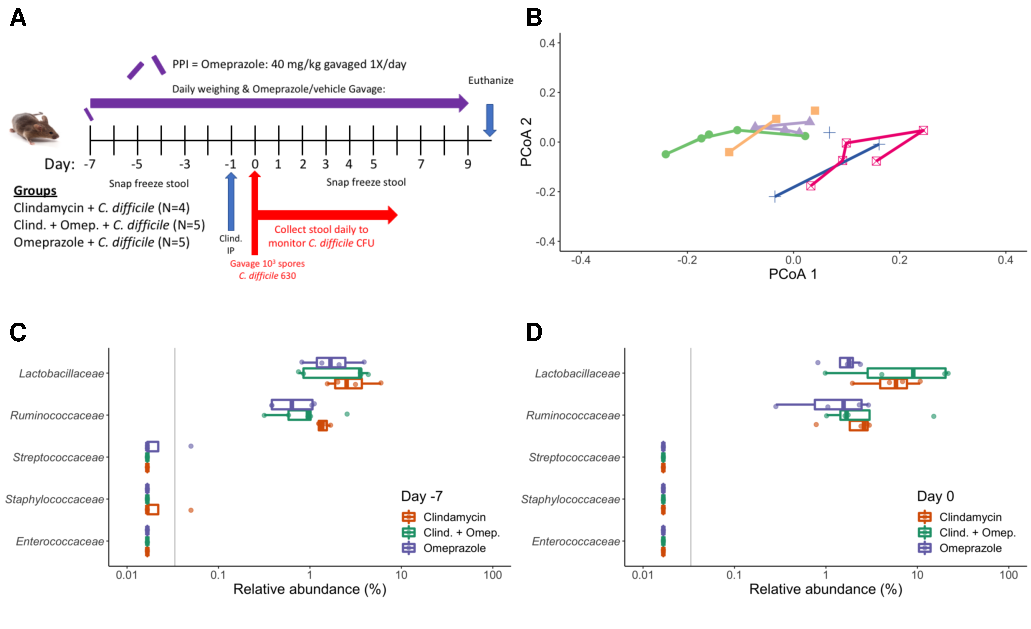
\includegraphics{figure_1.pdf} \textbf{Figure 1. PPI treatment had
minimal impact on the murine fecal microbiota} A. Mouse experiment
timeline and logistics. Stools for 16S rRNA sequencing analysis were
collected on the days that are labeled (Day -7, -5, -3, -1, 0, 1, 2, 3,
4, 5, 7, 9). B. Principal Coordinates Analaysis (PCoA) of Bray-curtis
distances from stool samples for all treatment groups during the intial
7 days of treatment with the PPI omeprazole or vehicle cluster together
and do not chage much over time. C. Relative abundances of families
previously associated with PPI use in humans do not change much over the
16-day course of treatment with PPIs (7 days before \emph{C. difficile}
challenge through 9 days post \emph{C. difficile} challenge). D. PCoA of
stool samples collected before and 1 day after antibiotic treatment,
demonstrating the fecal microbiota of mice treated with clindamycin
starts to separate from the rest of the samples.

\newpage

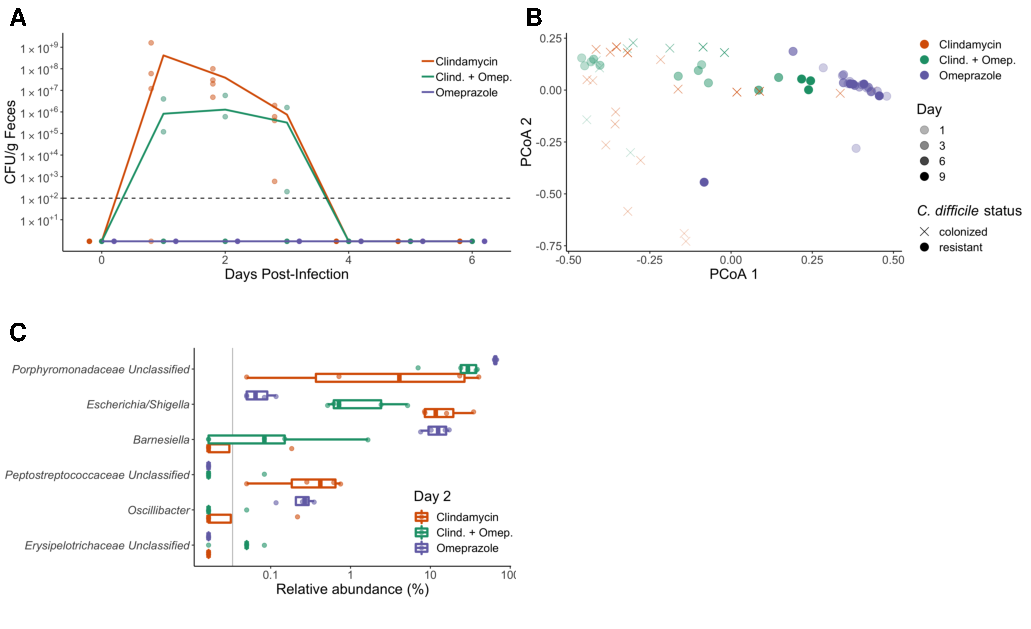
\includegraphics{figure_2.pdf} \textbf{Figure 2. PPI treatment alone
does not promote CDIs in mice} A. C. difficile CFUs/g stool measured
each day post C. difficile challenge for clindamycin, clindamycin/PPI,
and PPI-treated mice. Lines represent the mean CFU/g for each treatment
group while points represent CFU/g for individual mice within each
group. B. PCoA of stool samples collected after antibiotic treatments.
C. Genera significantly associated with treatment groups for samples
across all sequenced timepoints. D. Families significantly associated
with treatment groups for samples across all sequenced timepoints. C,D
data were analyzed by Kruskal-Wallis test with a Benjamini-Hochberg
correction for multiple comparisons.

\newpage

\includegraphics{figure_s1.pdf} \textbf{Figure S1. Previous human
PPI-associated families fluctuate over time with no overall trend in
either direction} Relative abundance over time for Lactobacillaceae (A)
and Ruminococcaceae (B), 2 of the PPI-associated familes from human PPI
studies across all 3 treatment groups. Each point represents the
relative abundance for an individual mouse


\end{document}
